\section{Results and Discussion}

\subsection{Baseline Noise Floor and Thermodynamic Correlation}
Following the initial transient dissipation, the baseline observation revealed a slow macroscopic environmental drift, as captured in Fig. \ref{fig:timeseries_T} and Fig. \ref{fig:timeseries_RH}. 
The temperature channel exhibited a linear positive slope of $+0.0043^\circ$C/min ($R^2 = 0.991$), attributed to the gradual accumulation of micro-environmental heat. 
Concurrently, the relative humidity (RH) channel demonstrated a highly correlated negative slope of $-0.0100$ \%RH/min ($R^2 = 0.980$). 

\begin{figure}[htbp]
\centering

\includegraphics[width=\columnwidth]{./assets/T/timeseries_plot.png}
\caption{Baseline time-series observation of the temperature channel demonstrating the positive macroscopic thermal drift prior to detrending.}
\label{fig:timeseries_T}
\end{figure}

\begin{figure}[htbp]
\centering
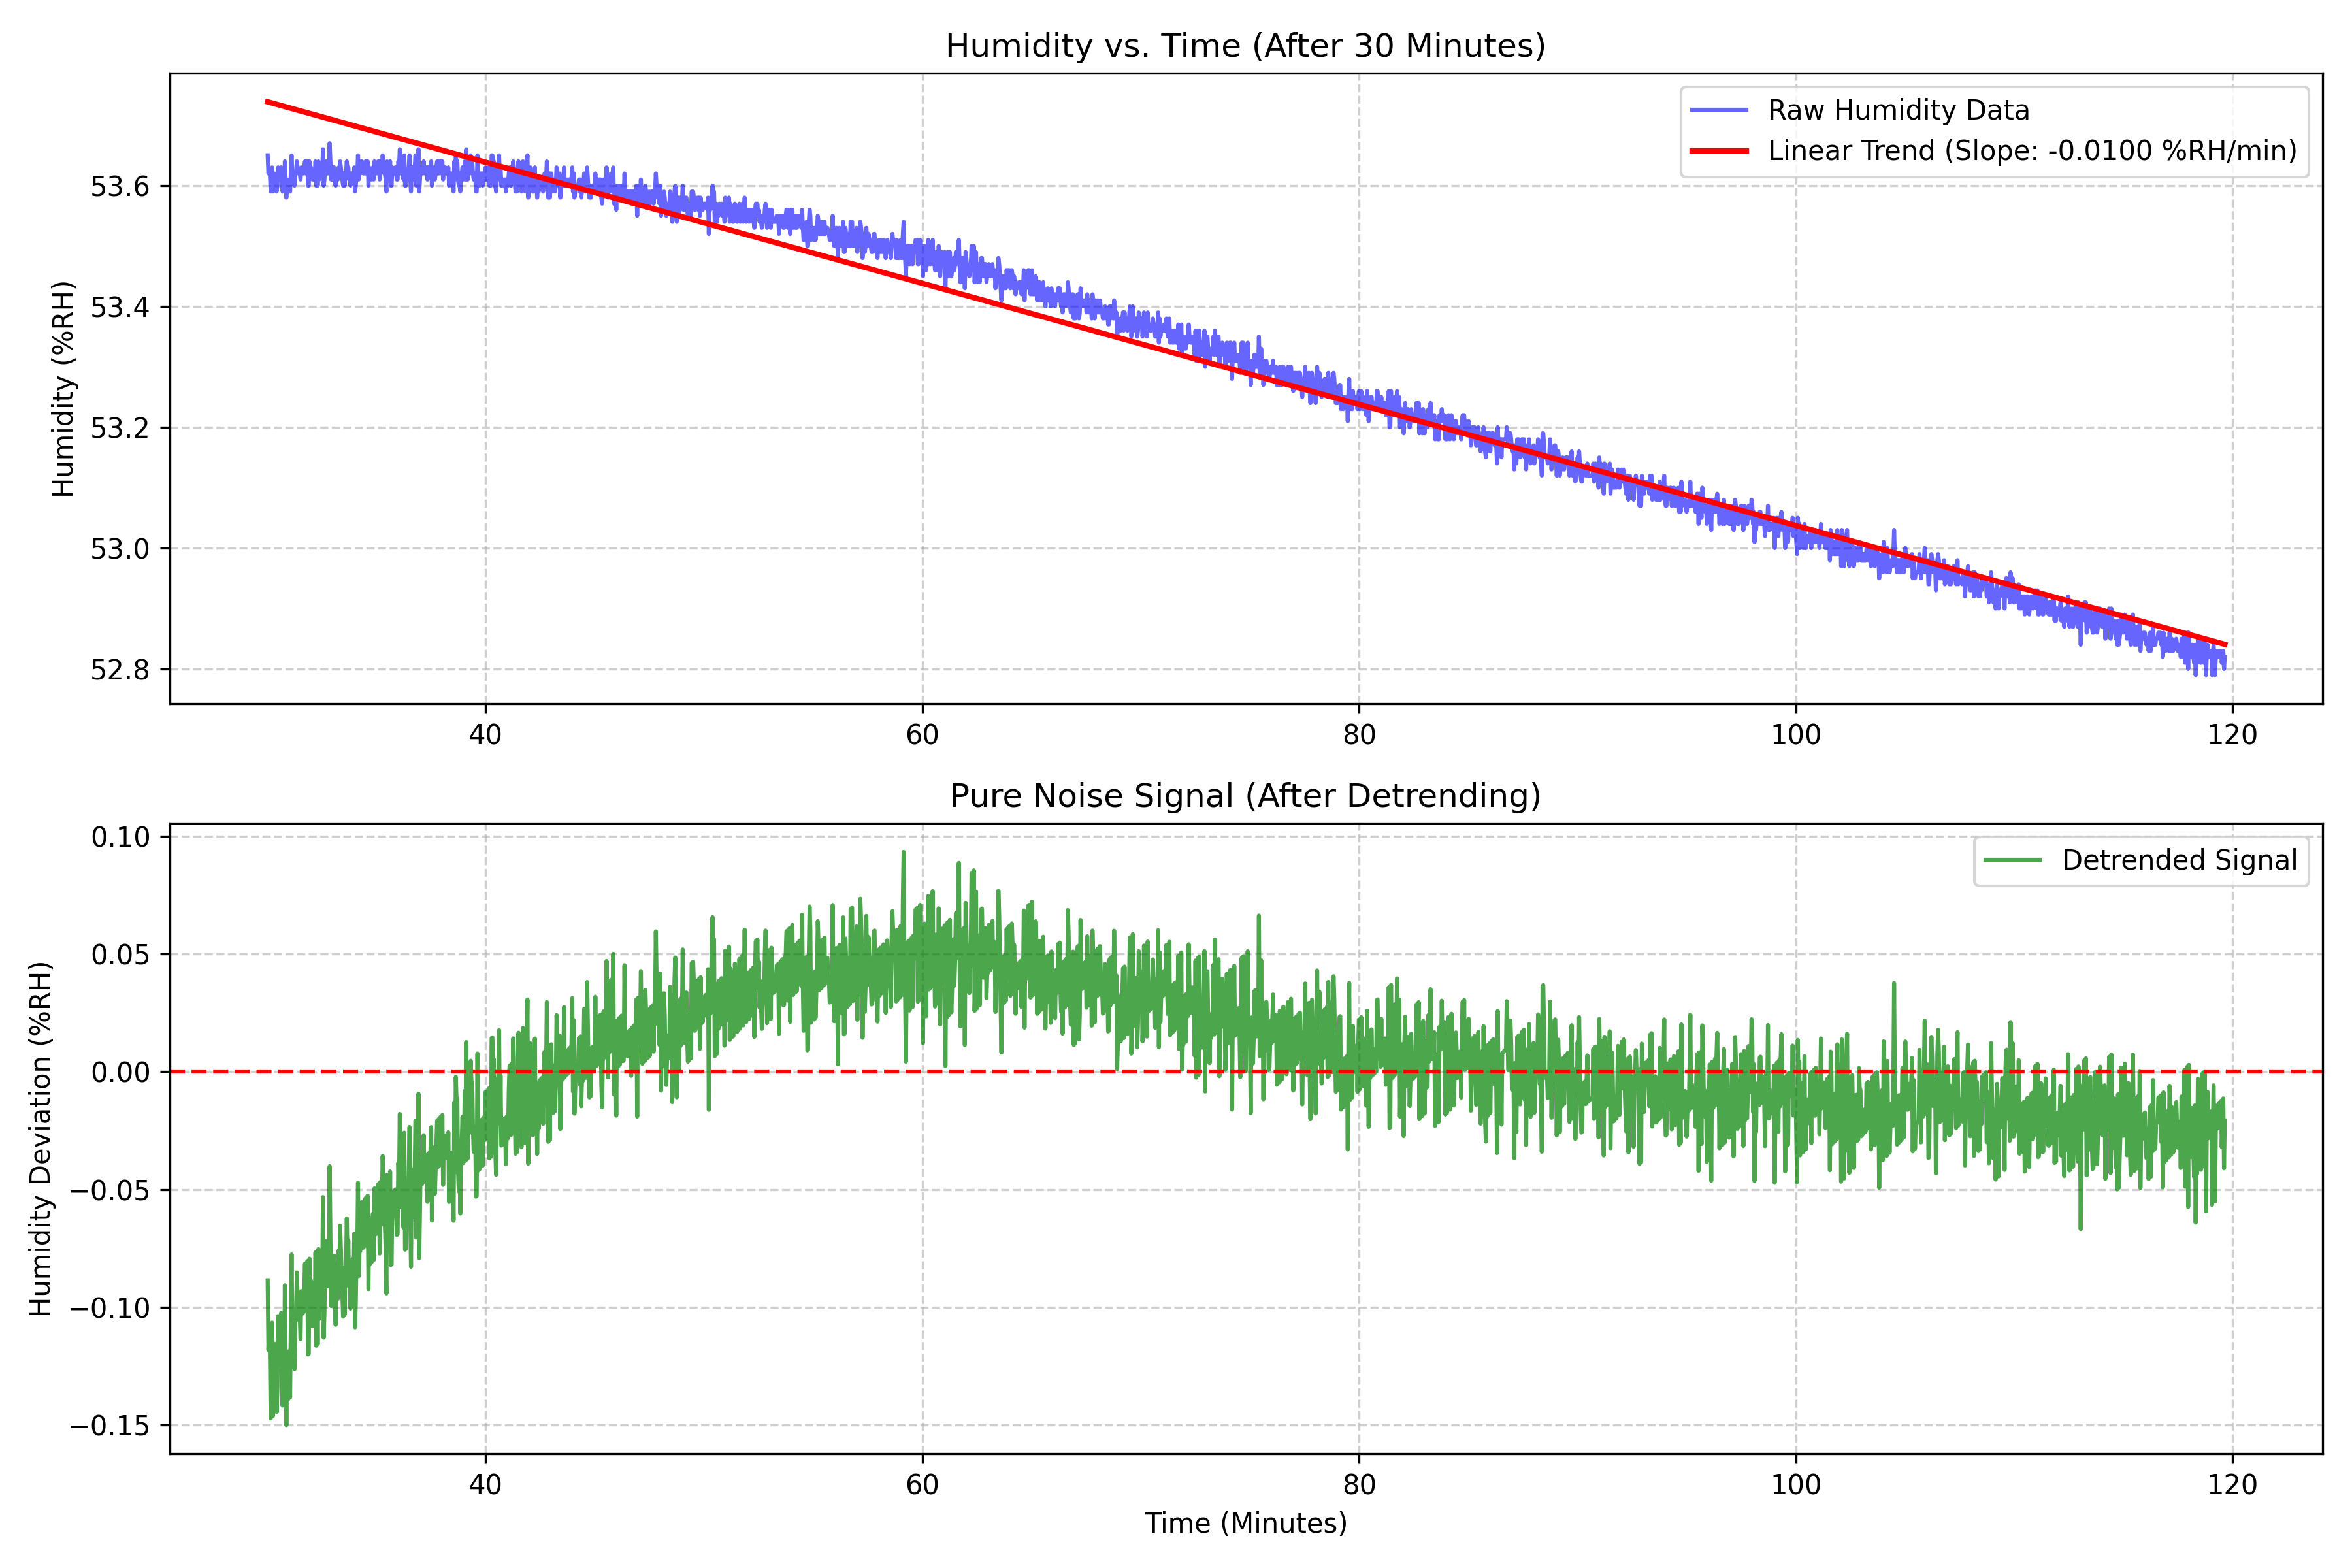
\includegraphics[width=\columnwidth]{./assets/RH/timeseries_plot.png}
\caption{Baseline time-series observation of the relative humidity channel demonstrating the inverse negative psychrometric drift.}
\label{fig:timeseries_RH}
\end{figure}

This behavior visually and mathematically confirms the inverse psychrometric relationship dictated by thermodynamics; 
at a constant absolute vapor pressure, an increase in sensible heat proportionally reduces relative humidity. 
Upon isolating this macroscopic drift via detrending, the true statistical means were established at $\mu_T = 30.7550^\circ$C and $\mu_{RH} = 53.2896$ \%RH, 
with isolated pure standard deviations (noise floors) of $\sigma_T = 0.0108^\circ$C and $\sigma_{RH} = 0.0370$ \%RH.

\subsection{Quantization Limits vs. Analog Front-End Noise}
To ascertain the physical origin of the measured uncertainty, 
the empirical noise floors were compared against the theoretical digital resolution of the sensor's 20-bit Analog-to-Digital Converter (ADC). 
The Least Significant Bit (LSB) quantization step for temperature is given by:
\begin{equation}
1 \text{ LSB}_T = \frac{200}{2^{20}} \approx 0.0001907^\circ\text{C}
\end{equation}
For the humidity channel, based on standard conversion parameters \cite{aht10_datasheet}, the resolution is:
\begin{equation}
1 \text{ LSB}_{RH} = \frac{100}{2^{20}} \approx 0.0000954\,\%\text{RH}
\end{equation}
The ratio of the measured noise floor to the quantization step demonstrates that the physical noise is $56.8\times$ larger than the digital limit for temperature ($0.0108 / 0.0001907$), 
and a substantial $388\times$ larger for humidity ($0.0370 / 0.0000954$). 
This strong quantitative evidence suggests that the precision bottleneck is primarily governed by the analog front-end (the capacitive polymer and silicon architecture) and thermodynamic fluctuations, rather than the digital bit depth. 
Consequently, transmitting raw, unfiltered data introduces severe measurement uncertainty, supporting the necessity of dedicated digital signal conditioning.

\subsection{EMA Filter Optimization via Cost Function}
Given the disparate physical properties of heat transfer versus moisture diffusion, 
the filter parameters required independent mathematical optimization. 
Evaluation of the objective function $J(\alpha)$ defined in \eqref{eq:cost_func} yielded distinct parabolic minima for each physical channel.

\begin{figure}[htbp]
\centering

\includegraphics[width=\columnwidth]{./assets/T/cost_function_optimization.png}
\caption{Cost function minimization for the temperature channel, indicating an optimal $\alpha_T = 0.1494$.}
\label{fig:cost_T}
\end{figure}

\begin{figure}[htbp]
\centering
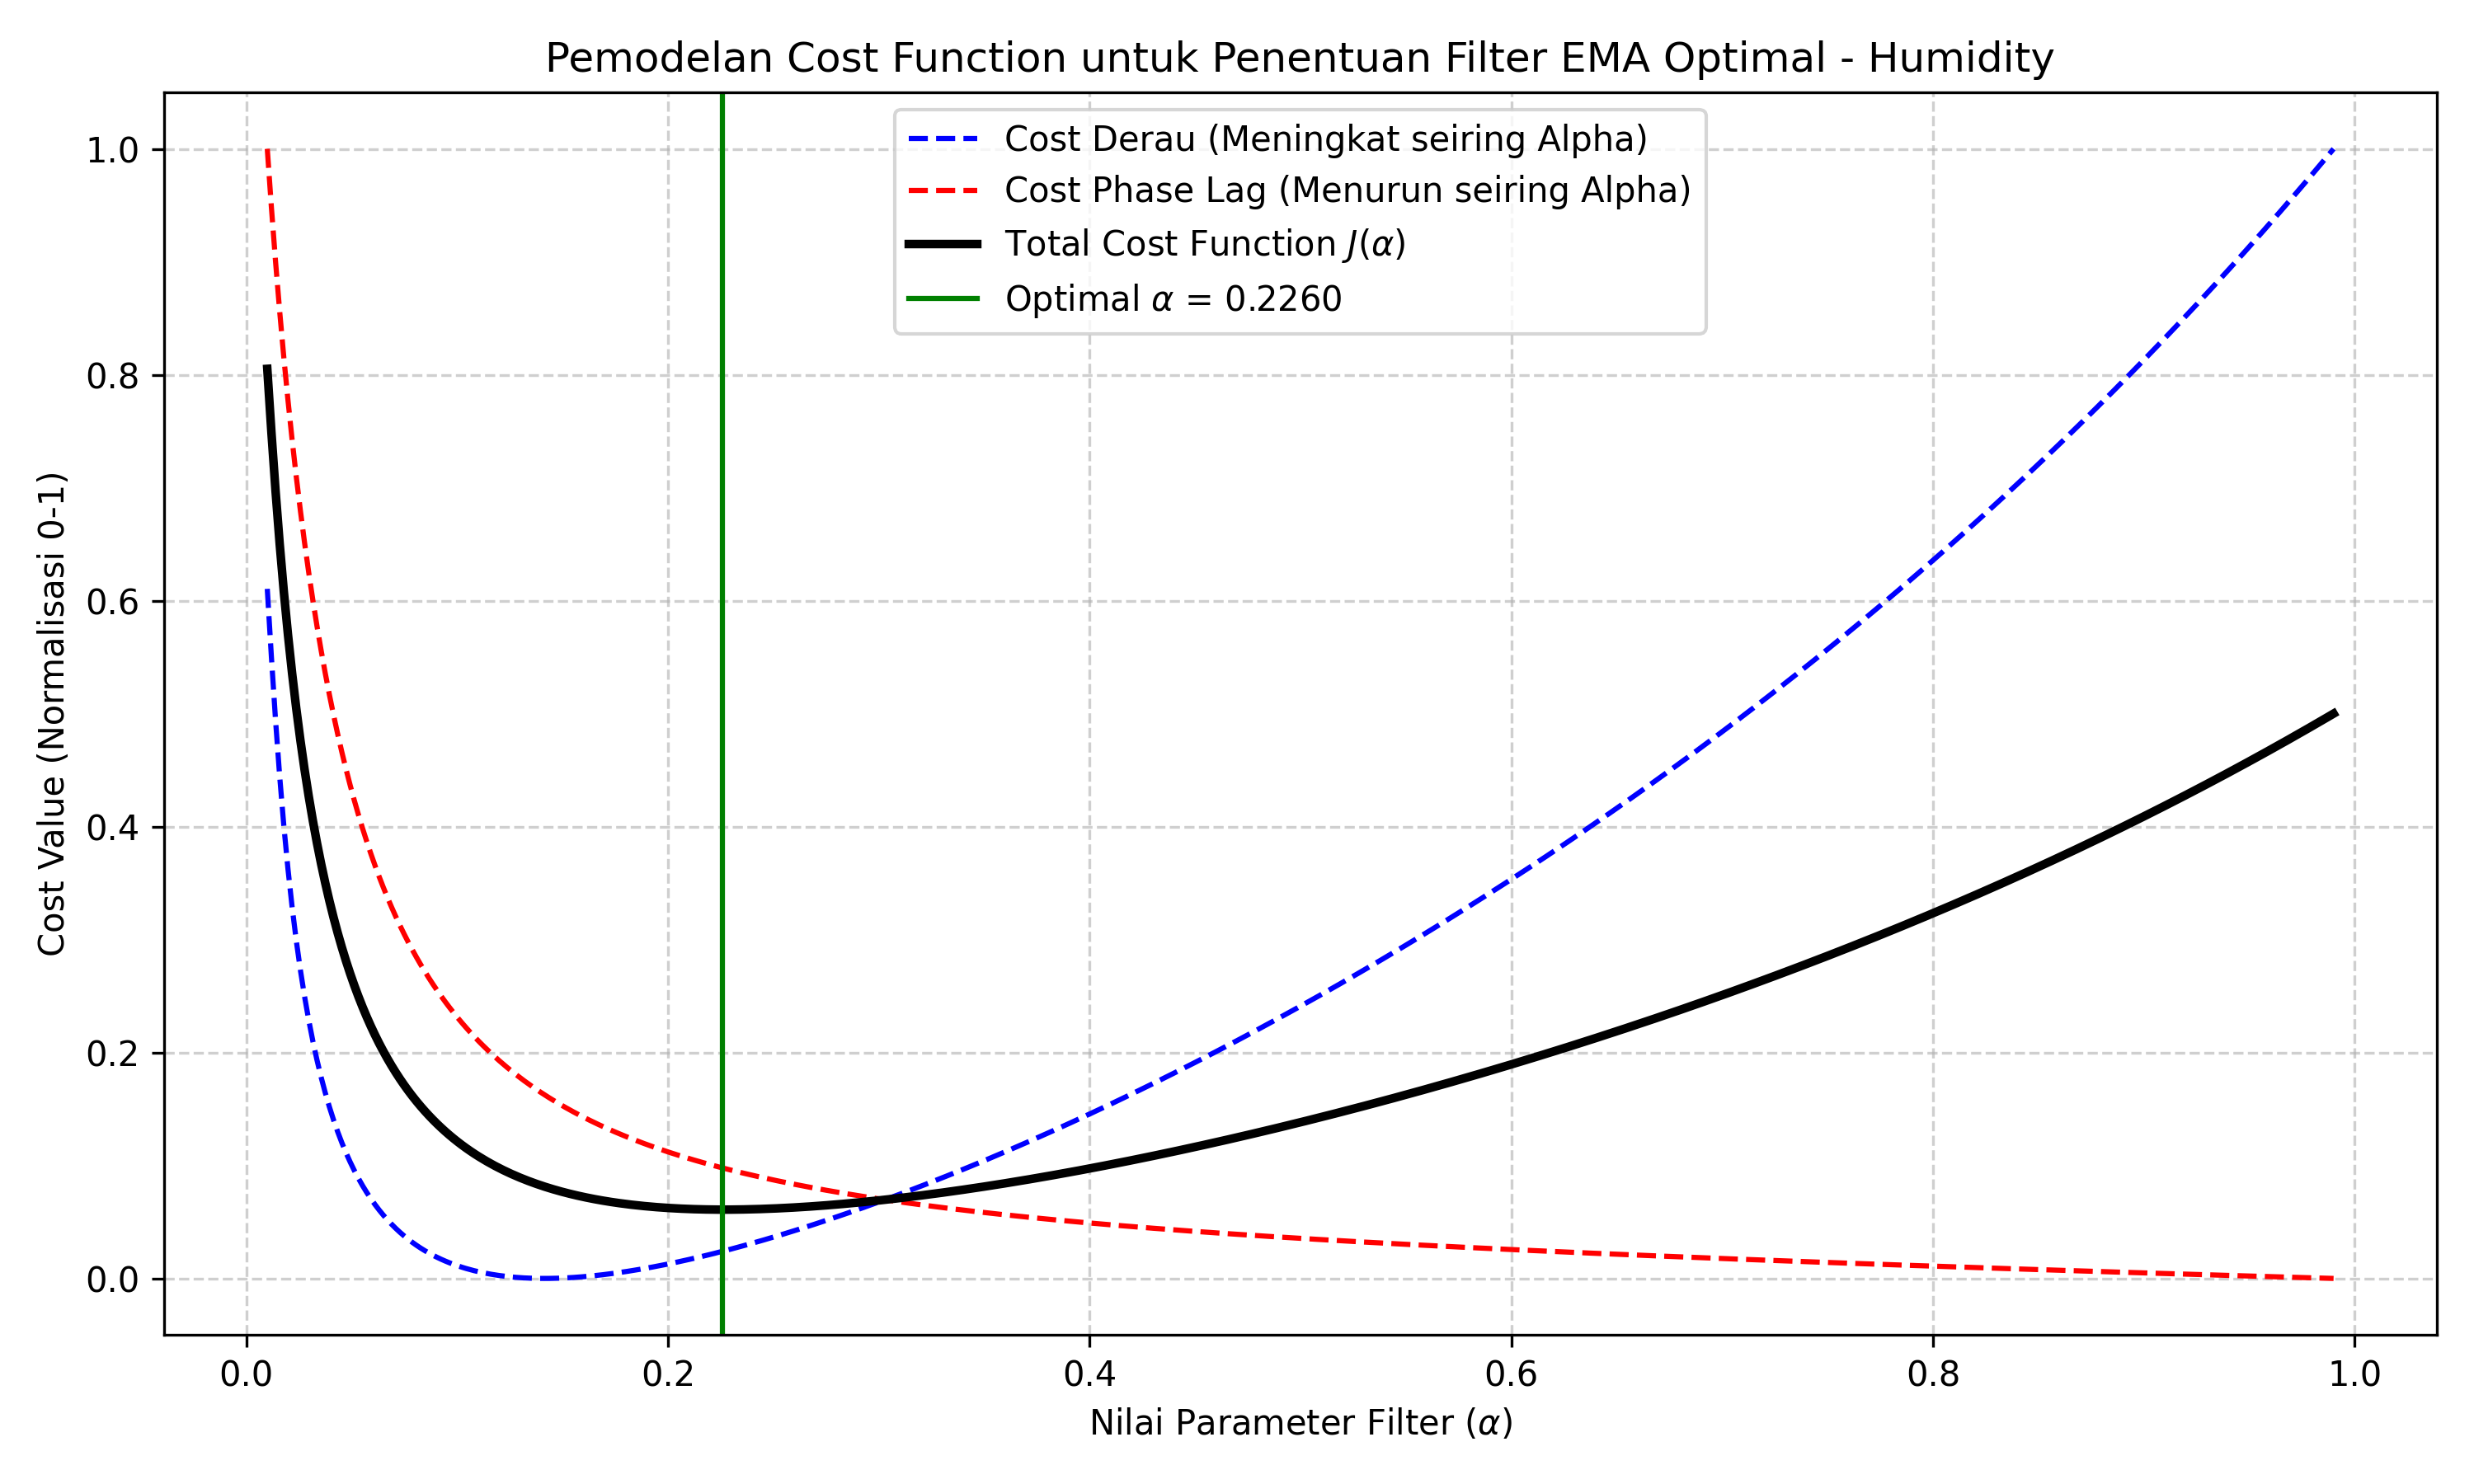
\includegraphics[width=\columnwidth]{./assets/RH/cost_function_optimization.png}
\caption{Cost function minimization for the relative humidity channel, indicating an optimal $\alpha_{RH} = 0.2260$.}
\label{fig:cost_RH}
\end{figure}

The baseline penalty weights ($W_1 = W_2 = 0.5$) utilized in the Cost Function were established under a neutral parity assumption, 
granting equal priority to steady-state noise suppression and transient response fidelity for environmental data-logging applications. 
While advanced multi-objective frameworks (such as Pareto fronts or Bayesian optimization) could map broader weighting trajectories, 
a balanced parity baseline provides a clear and reproducible design starting point. 
Under this configuration, as depicted in Fig. \ref{fig:cost_T} and Fig. \ref{fig:cost_RH}, numerical minimization established the optimal smoothing factors at $\alpha_T = 0.1494$ and $\alpha_{RH} = 0.2260$. 
The significantly higher $\alpha$ value for the RH channel reflects the faster intrinsic transient dynamics of humidity within this experimental boundary, allowing for more aggressive smoothing without proportionally sacrificing phase lag. 
The optimized filter parameters yield a theoretical noise standard deviation ($\sigma$) reduction of $71.6\%$ (corresponding to a $91.9\%$ variance attenuation) for temperature, and $64.3\%$ ($87.3\%$ variance attenuation) for humidity.

To rigorously test the stability and responsiveness of the optimization framework against shifting design priorities, 
a sensitivity analysis was conducted by adjusting the penalty weights to prioritize transient response fidelity ($W_1 = 0.3$ for noise variance and $W_2 = 0.7$ for phase lag). 
Executing the numerical minimization under this lag-prioritized configuration shifted the optimal smoothing factors upward to $\alpha_T = 0.2555$ for temperature and $\alpha_{RH} = 0.2967$ for relative humidity. 
This systematic upward migration mathematically confirms the elasticity of the Cost Function: as the operational penalty for transient delay increases, the system autonomously increases $\alpha$ to track rapid physical changes more aggressively, 
demonstrating that the framework can be seamlessly tailored to alternative embedded architectures (such as closed-loop control systems).

\subsection{Quantitative Evaluation of Phase Lag}
The transient phase lag was quantitatively evaluated across a critical temporal window (Minutes 3.0 to 6.0) following the physical step input.

\begin{figure}[htbp]
\centering

\includegraphics[width=\columnwidth]{./assets/T/transient_overall_plot.png}
\caption{Overall transient response of the temperature channel post-injection.}
\label{fig:transient_T}
\end{figure}

\begin{figure}[htbp]
\centering
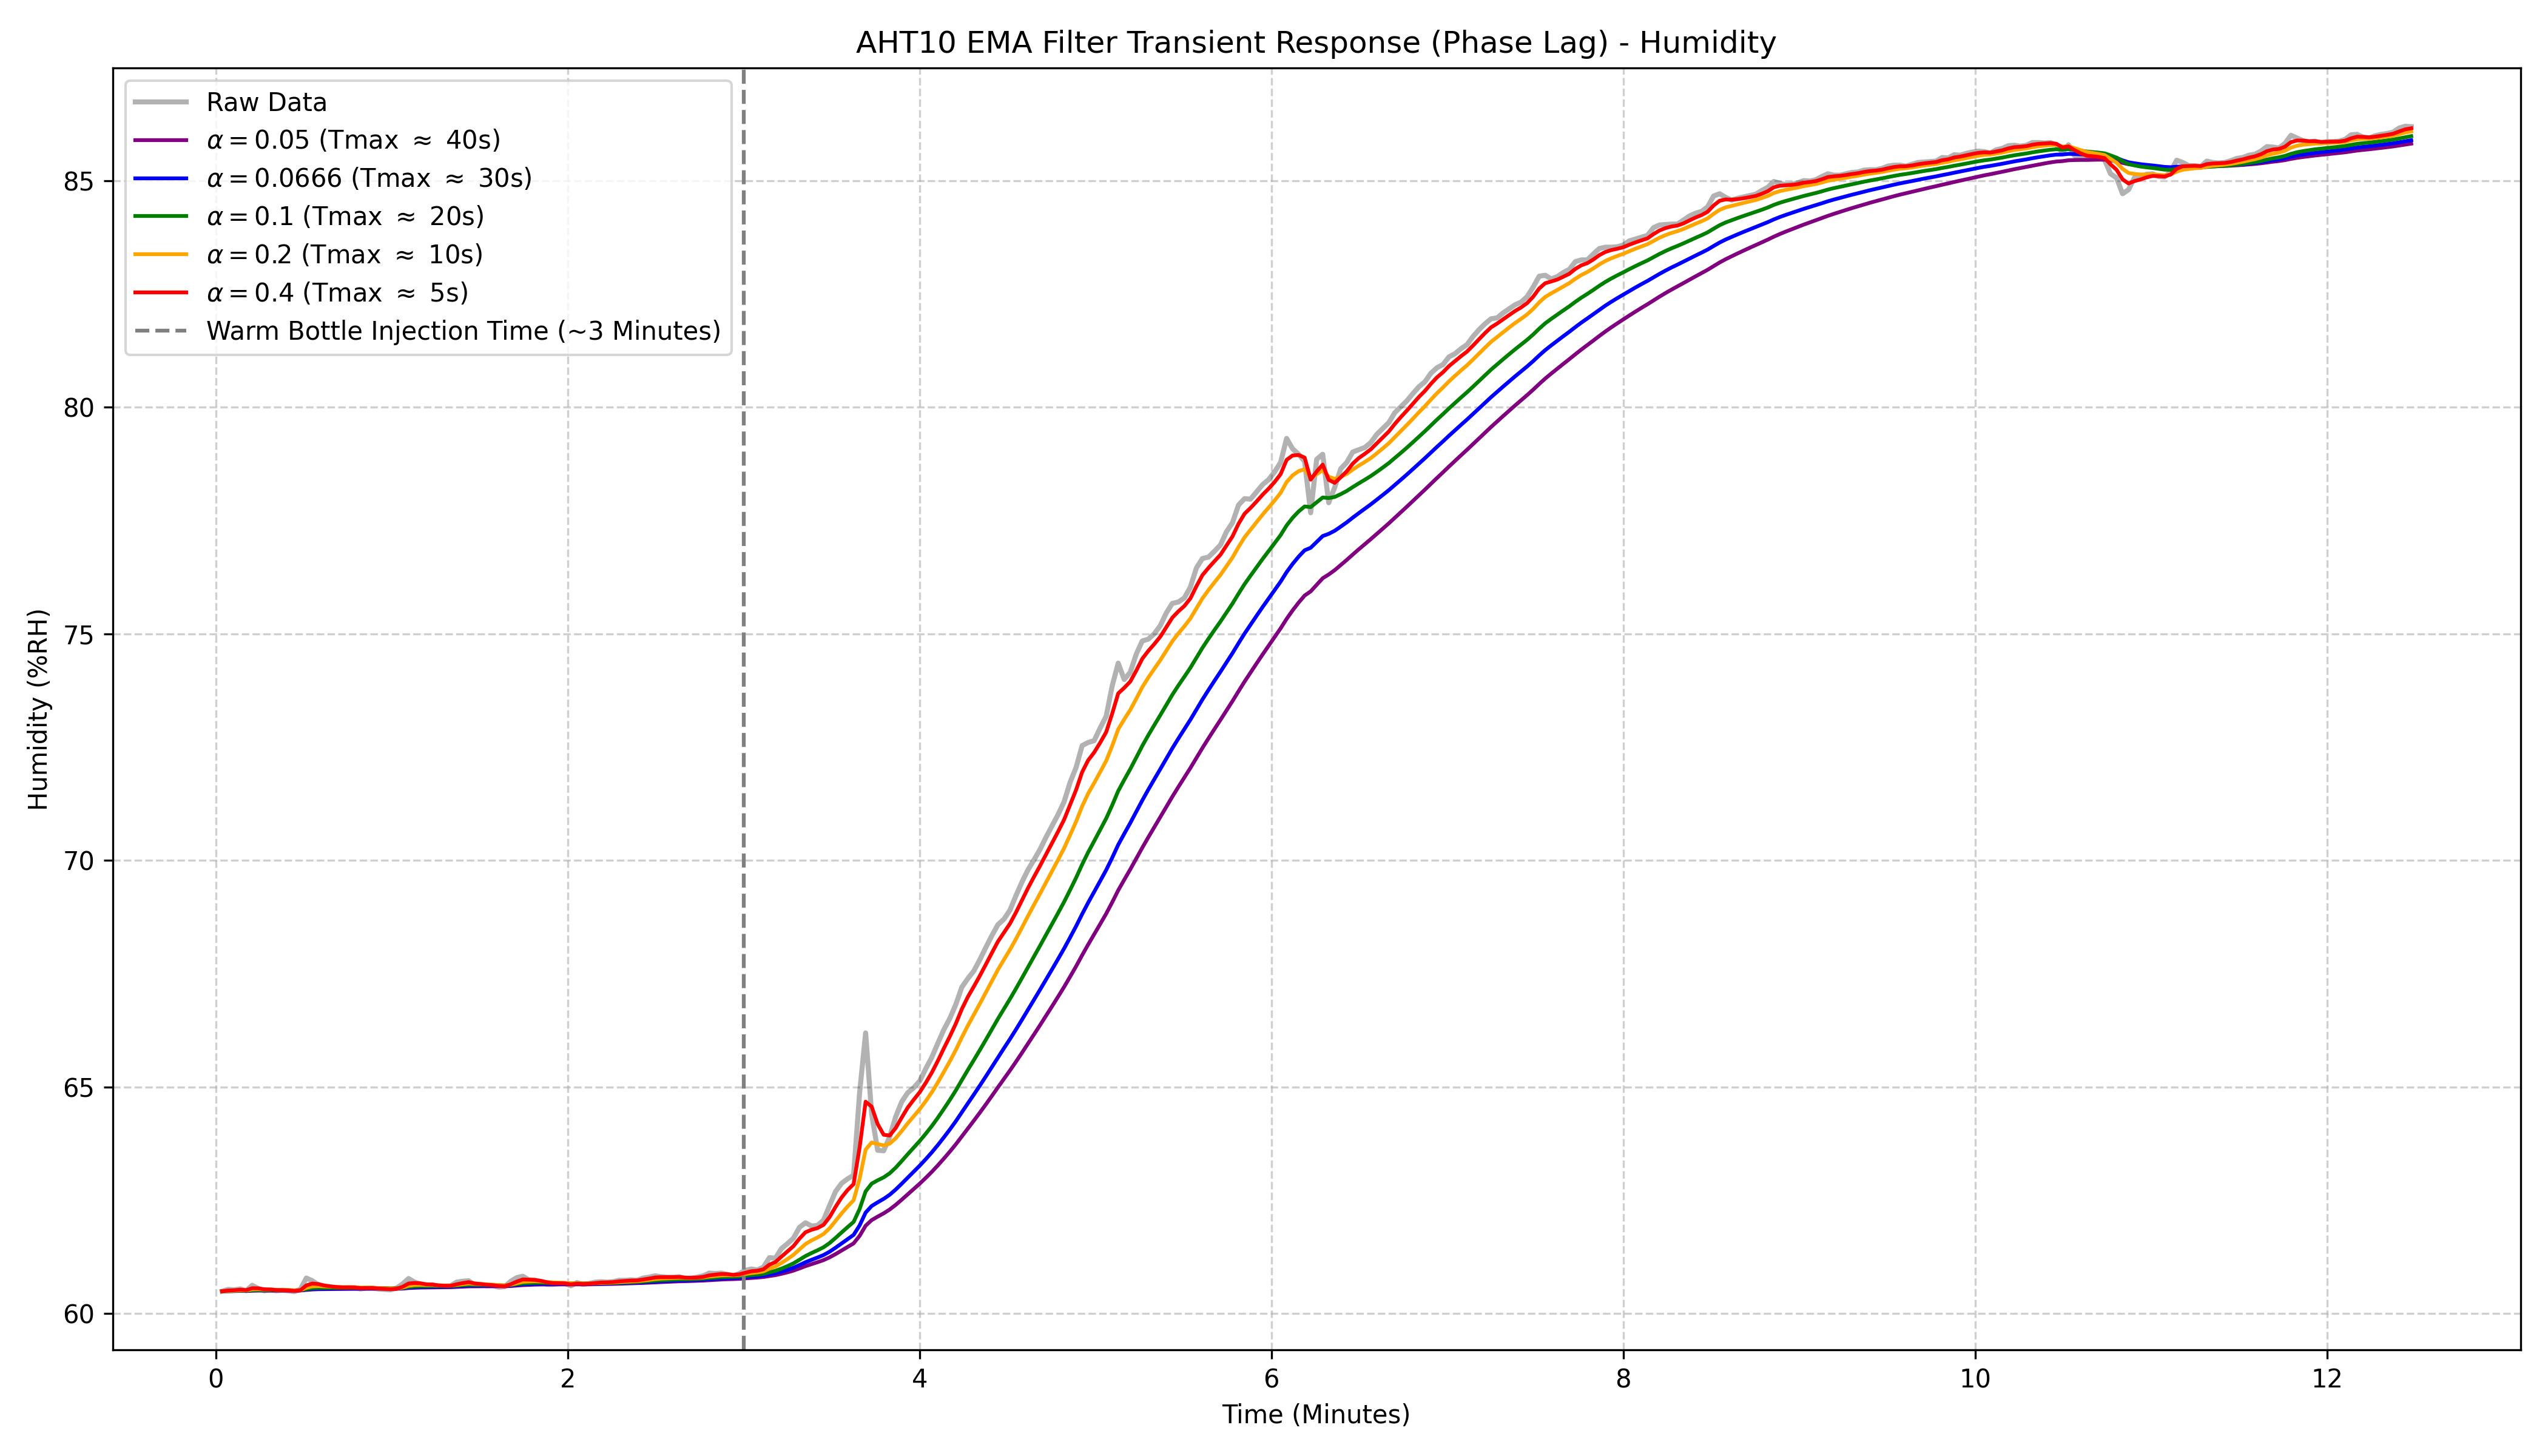
\includegraphics[width=\columnwidth]{./assets/RH/transient_overall_plot.png}
\caption{Overall transient response of the relative humidity channel post-injection.}
\label{fig:transient_RH}
\end{figure}

Applying $\alpha_T = 0.1494$ reduced the Root Mean Square Error (RMSE) to $0.0771^\circ$C with a Maximum Lag Error of $0.1333^\circ$C, occurring at exactly $3.39$ minutes post-injection (Fig. \ref{fig:transient_T}). 
For humidity (Fig. \ref{fig:transient_RH}), applying $\alpha_{RH} = 0.2260$ yielded an RMSE of $0.7560$ \%RH and a Max Lag of $2.3984$ \%RH, locking at $3.69$ minutes. 
The locking of maximal lag early in the transient window confirms the characteristic low-pass behavior of the filter in absorbing initial shock responses before adapting to the continuous physical change.

Translating these discrete variables into continuous physical time constants ($\tau$) using the relationship $\tau = -\Delta t / \ln(1-\alpha)$ yields $\tau_T \approx 12.67$\,s and $\tau_{RH} \approx 8.00$\,s. 
Crucially, the empirically derived $\tau_{RH}$ is mathematically identical to the intrinsic ``typical response time'' ($t_{63\%} = 8$\,s) specified by the AHT10 manufacturer \cite{aht10_datasheet}. 
Concurrently, $\tau_T$ falls perfectly within the established $5$--$30$\,s limit for thermal response. 
This serves as a definitive cross-validation: the objective, data-driven optimization of the cost function independently converged upon the physical thermodynamic limits of the hardware itself.

\subsection{Experimental Limitations and Gap Analysis}
While the empirical models present robust cross-validation against the physical hardware specifications, the methodological framework contains intrinsic metrological limitations. 

First, the deterministic hardware polling interval ($\Delta t = 2.051$\,s), while vital to strictly cap the SoC Joule heating below $0.1^\circ$C, limits the Nyquist frequency to $f_N \approx 0.243$\,Hz. 
Consequently, any high-frequency microclimate turbulence exceeding this limit cannot be reconstructed and will alias into the baseband, representing a deliberate design compromise that prioritizes long-term thermal stability over high-frequency dynamic capture.

Second, the physical transient injection utilized in Protocol II (warm water at $40^\circ$C--$50^\circ$C) deviates from an ideal mathematical Heaviside step function. 
The finite heat transfer rate dictates the temperature gradient, preventing an instantaneous physical change. 
Furthermore, the injection introduces not only sensible heat but also latent heat in the form of water vapor. 
This instantaneous surge in absolute humidity induces microscopic condensation on the AHT10's capacitive polymer membrane, where subsequent mechanical absorption and desorption phases introduce a physical inertia that overlaps with algorithmic phase lag. 
Therefore, the recorded RMSE and Max Lag Error metrics reflect the specific boundary constraints of this experimental setup and the sensor's mechanical membrane inertia. 

Finally, regarding the objective optimization framework, the baseline parity assumption ($W_1 = W_2 = 0.5$) provides a balanced starting point for environmental data logging. 
Preliminary sensitivity evaluations indicate that shifting the weights (e.g., favoring noise reduction with $W_1 = 0.7, W_2 = 0.3$) yields a more conservative smoothing factor ($\alpha$ decreases), reducing steady-state variance at the expense of a prolonged transient time constant. 
Future investigations could extend this optimization via multi-objective Pareto mapping, expand the metrological pipeline across alternative multi-sensor architectures (e.g., BME280, SHT31), and incorporate Type A/B expanded uncertainty frameworks to generalize these findings further.
